
%%%%%%%%%%%%%%%%%%%%%%%%%%%%%%%%%%%%%%%%%%%%%%%%%%%%%%%%%%%%%%%%%%%%%%%%%%%%%%%%%%
%%% Navigation
%%% 
%%% Section 1 : Survey of Algorithms
%%% 	Subsection 1.1 : Classes of Algorithms
%%% Section 2 : Potential Fields
%%%	Section 3 : GODZILA
%%% mention that one aspect of navigation is vertically constrained spaces, connect to next chapter
%%%%%%%%%%%%%%%%%%%%%%%%%%%%%%%%%%%%%%%%%%%%%%%%%%%%%%%%%%%%%%%%%%%%%%%%%%%%%%%%%%
\chapter{Navigation} \label{ch:navigation}

%%% What is navigation? %%%
% Make this section less colloquial.
Navigation is the task of generating a series of commands that allow a robot to transit from its current pose
to some goal pose. This task encompasses a number of subtasks such as path planning, environment sensing, and obstacle
avoidance. As a robot transits through space from its current to goal pose, it necessarily visits a series
of intermediate poses the choice of which depends on its kinematic constraints and the constraints of the environment it transits through. 
Collectively, this set of poses as a time sequence is known as a path. 
The spacial region in which the robot operates is known as the task space and all kinematically feasible configurations is known as the
configuration space.  Typically, the environment a robot traverses is not free space but also contains obstacles 
which constrain the paths which can be taken to the goal. While in some 
controlled environments the location of obstacles can be known \textit{a priori} and supplied to the robot in the form of a map, often the
robot will have the task of creating a map which describes the location of these obstacles. In some situations, ``global" 
sensors can view the entire environment within which the robot will operate and can capture all of the constraints while in others (especially
in the case of mobile robots) only ``local" sensors mounted to the robot are available to detect environmental limitations
to the robot's path as they are encountered. Even more challenging is the case where the environmental obstacles are not
static but are moving adding a time varying element to the obstacle avoidance problem.

% In the first place that you mention the categories, you can clarify that the categories are not mutually exclusive,
% but that algorithms are classified into combinations of categories.

% Algorithms that solve the navigation problem are sometimes described according to four major categories.

% Here's one way to split up things:
Algorithms that solve the navigation problem are sometimes described according to four major categories (though there are many
other categories with which these algorithms could be described with). These categories are not mutually exclusive, and algorithms
are commonly attributed with multiple classifications.
The first two, known as global or local, speak to the amount
of spatial data or time horizon considered when planning a solution. If only a short time horizon or occlusions in the immediate
spatial region are accounted for, then the algorithm is considered local, otherwise it is thought of as global.
The other two deal with how the spaces or paths are represented, continuously or discretely. If the algorithm breaks
up these spaces into finite resolution pieces, then it is discrete. Continuous algorithms choose some sort of parameterization
to the spatial or environmental constraints using a model. Often algorithms are some mixture of all of these four categories.

The algorithm used for navigation in this thesis is the GODZILA navigation algorithm, 
which can be categorized as a local continuous algorithm based on the potential fields navigation strategy. 
While in many environments GODZILA solves the navigation problem, it can also be used in conjunction with global algorithms
that can plan way points to the goal without having to consider the detailed local environment.

%%% Addendum's %%%
In the design on the obstacle avoidance algorithm for a robot, it is important to consider how different local sensors 
can affect the choice of navigation algorithm. The Nao humanoid platform
used in this thesis is equipped with two sonar sensors for obstacle detection. Details on these are given in Chapter \ref{ch:platform}.
These sensors have a broad angular range and cannot provide information about where within this cone obstacles are located.
This enables the robot to avoid colliding with objects directly in front of it but might cause the obstacle avoidance algorithm
to preclude the discovery of possible paths (e.g., narrow corridors between obstacles).
Conversely, scanning laser rangefinders (such as the one mounted to the Nao and described in Chapter \ref{ch:platform}) have a
very high degree of angular resolution and provide hundreds of range measurements. This allows for a more accurate description
of environmental occlusions allowing more paths to be considered for traversal.
% [Insert picture of sonar cones vs lasers.]
\begin{figure}
	\centering
	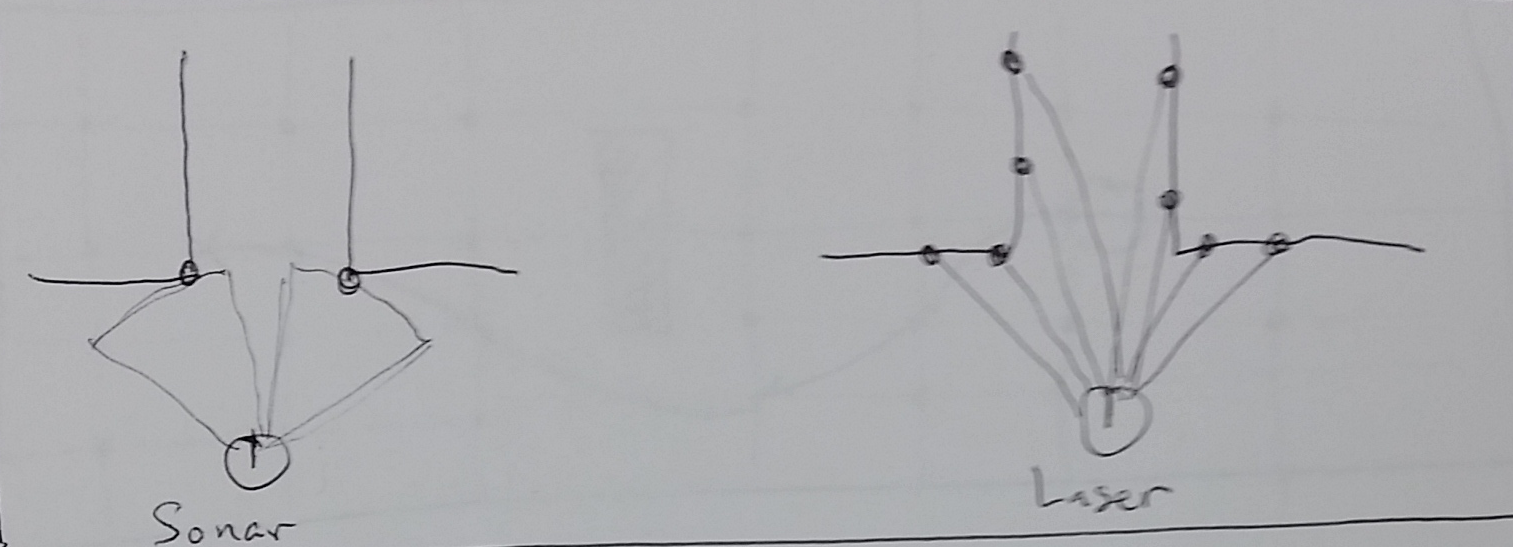
\includegraphics[width=\textwidth]{sonar_lidar_rough1.png}
	\caption
	{Sonar sensors are typically preferred when needing to detect the presence of an obstacle without
	 needing precise position information. The location of a chair leg in the path of a robot would be
	 detected by sonar while not knowing its position in the sonar cone. Laser rangefinders have very
	 narrow beam width, typically requiring many of them to be effective at describing an environment.
	 If many measurements are available at high angular resolution, then they can be very effective at
	 describing the width of narrow apertures.}
	\label{fig:sonar_vs_lidar1}
\end{figure}

The notion of what objects in the environment occlude a path and which do not can be viewed as a function of the gait 
(or mode of locomotion) used by the robot. If the robot is restricted to a plane, such as the case in many ground vehicles,
then an object of similar size to the vehicle could prevent traversal through that position. If the robot can also fly then
that object may not present an impediment to proceeding towards the goal.
While still not transiting through that exact position in 3D space, the 2D projection of the path onto
the plane will appear to have moved through the obstacle. This can be though of in terms of a transformation of the obstacle set according to the different
motion modalities, making a 2D planner still applicable to the problem. In Chapter \ref{ch:crawl_gait},
a crawling gait for the Nao robot is considered which allows it to go under occlusions that it would otherwise need to plan
around.


\section{Algorithm Classifications}
Here some of the different notions common to navigation algorithms are explored. These classifications are sometimes useful
for the navigation engineer to think about as tools available to solve the navigation problem. While additional classifications
and subclassifications of algorithms can be considered, the following description is intended as a brief overview of the 
essential concepts.

\subsection{Global}
One approach to the navigation problem is to consider the entire task and configuration space of a problem when generating
a solution. For example, the task space of a robot arm might be the pose of the end effector and all of the occlusions
within that space. The configuration space would be the set of all valid joint angles that the arm can attain. Using this,
an algorithm can compute a time sequence of poses or movement commands that the robot should execute in order to bring it
from its current pose to the final pose. While this approach is ideal in the sense of generating a solution to the 
original problem, it has several practical disadvantages. One requirement of the algorithm is having a complete description 
of the task space. In many cases global knowledge of occlusions while planning is not available meaning that when new
obstructions are observed, the algorithm needs to replan the path. The other commonly encountered problem with these
algorithms is when the magnitude of the space to be planned through is so large that computing a solution cannot be done
in real-time.
% [Insert picture of global path and local directions.]
\begin{figure}
	\centering
	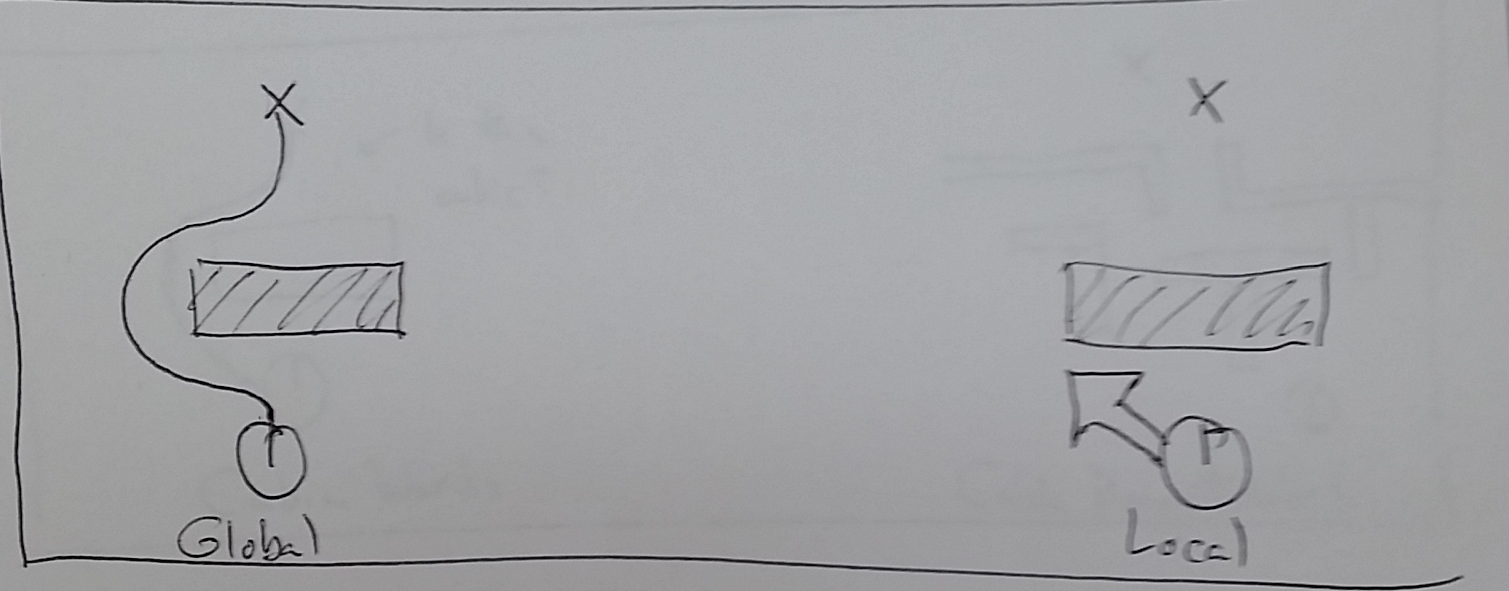
\includegraphics[width=\textwidth]{global_local_rough1.png}
	\caption
	{In global approaches, an entire path is planned to the goal before commanding the robot. In local 
	schemes, the robot is given commands calculated as a function of its position and the local environment and
	a complete path to the goal is typically precomputed. }
	\label{fig:global_vs_local1}
\end{figure}

\subsection{Local}
A different approach to the navigation problem is generating commands based only on the current information available 
or a short history about the environment. In the robot arm example, there might be a sensor such as a camera that
can detect objects that are obstructing the end effector from reaching the goal and instructs the arm to move around it.
Such algorithms usually have the advantage of being quick to compute as compared to their global counterparts because
they only have to consider a small subset of the task and configuration space. Their main disadvantage is that since they
only use such a limited amount of information, they can become trapped in local optima that do not allow the robot 
to achieve the desired pose.

%%% Continuous and Discrete %%%
\subsection{Discrete}
Orthogonal to the ideas of local and global path planning which deal with the scope of the time and space being considered
when generating navigation commands is how these spaces are represented. One way to represent the space is to break it
up into a set of discrete locations and then plan through that discretized representation. The task space for example could be divided into uniform 
spatial regions which an algorithm can consider visiting when planning a path. Alternatively, as with the robot arm example,
a finite set of movement commands can be considered and iterated through while generating a solution. 
Graph-based search algorithms such as  Dijkstra's algorithm or A* are examples of discrete solvers.
An advantage to this is that paths with complex shapes can be generated to accommodate difficult constraints. 
One point however to consider in this approach is how finely to resolve the task or configuration spaces. 
Coarser discretization can allow a solution to be computed rapidly but might miss more optimal solutions. 
% [Insert grid based path example.]
\begin{figure}
	\centering
	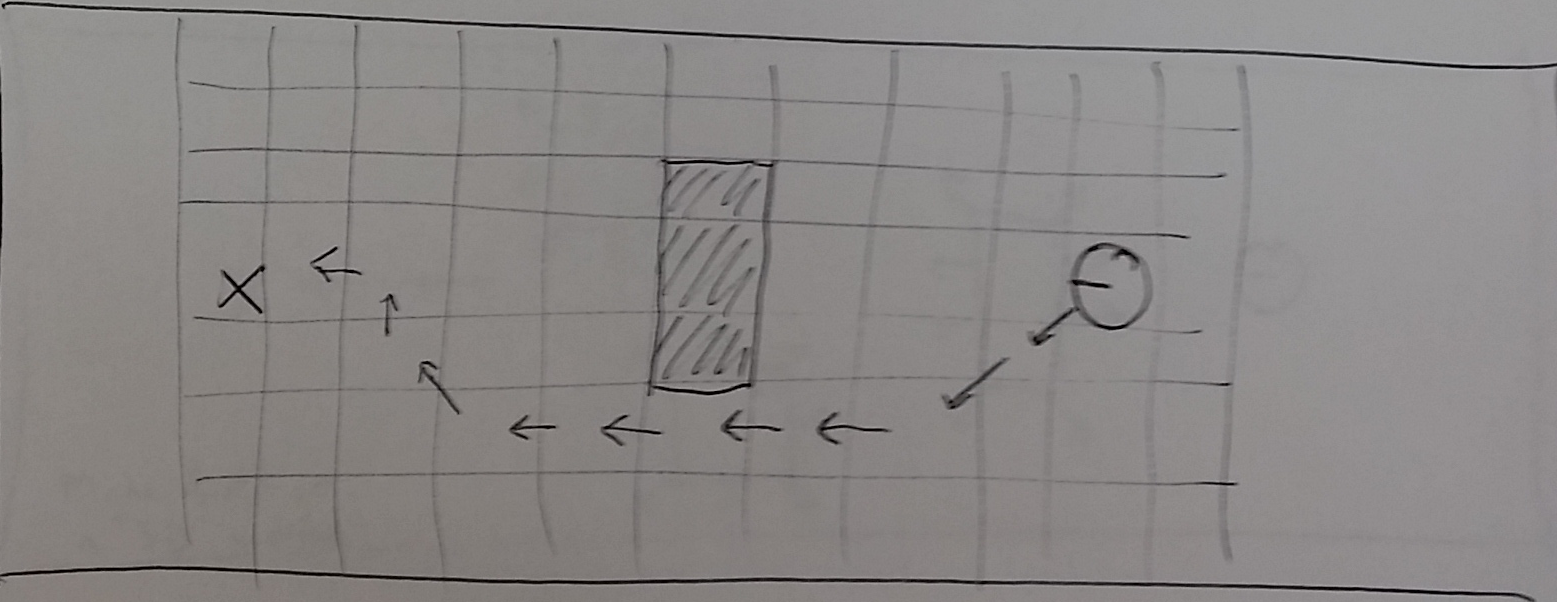
\includegraphics[width=\textwidth]{grid_world_rough1.png}
	\caption
	{The environment here is being represented as occlusions in a discrete grid of locations.
	This allows the robot to plan through successive locations to the goal using graph-based techniques.}
	\label{fig:grid_world1}
\end{figure}

\subsection{Continuous}
Continuous spatial representation avoids the problem of having to choose a discretization resolution. The movement commands or paths
are planned in a continuum allowing paths to take on intermediate values not available at a given discrete resolution.
Continuous representation instead has a different problem of paths needing to take on particular solution forms. A path
through the task space might be represented as a cubic spline from the current pose to the goal pose. This path has access
to the entire task space but may not be able to construct a path under complicated environments with many obstacles. Often
instead of using a single cubic, designers will use a series of cubics, the termination of one being the starting
position of the next, until the goal is reached. 
Alternatively, instead of restricting the path representation to a series of cubics, other trajectory forms can be
utilized as a library of representations such as higher-order polynomials, trigonometric functions, etc.
One example of such a planner is known as a ``maneuver-based" planner.
% [Insert figure than shows a successful cubic spline path and a maze where you couldn't use that.]  
\begin{figure}
	\centering
	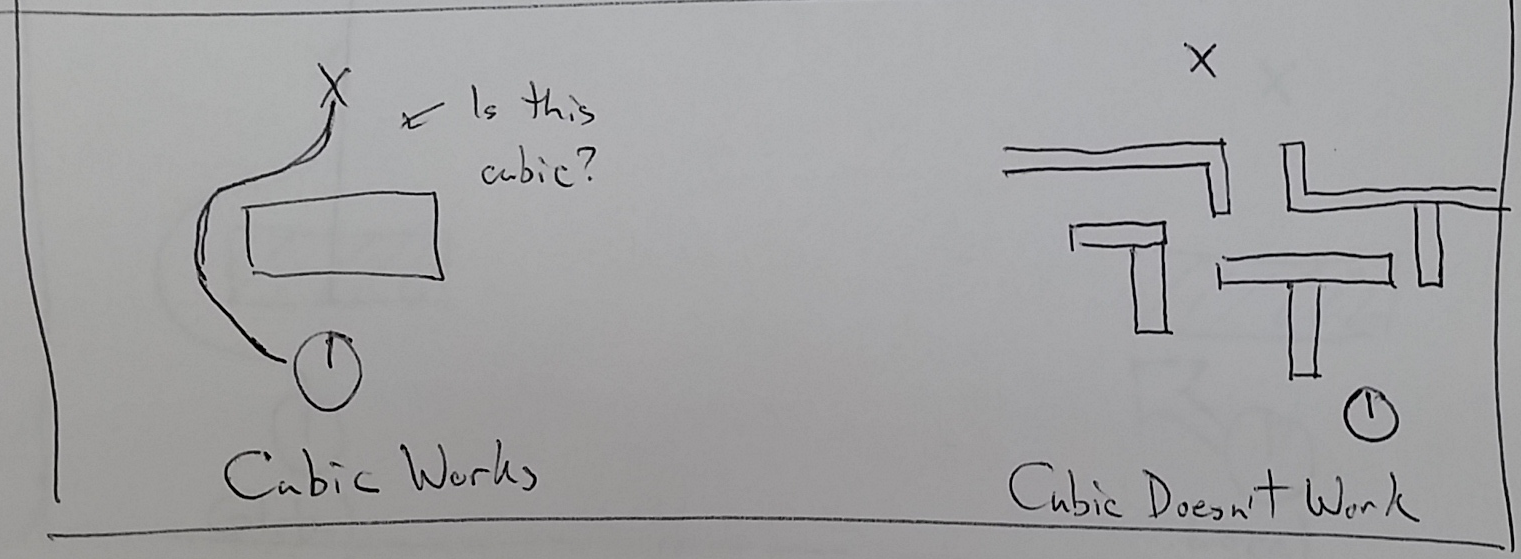
\includegraphics[width=\textwidth]{cubic_rough1.png}
	\caption
	{This figure shows two sample environments. On the left, the robot can follow a trajectory that takes
	a cubic form and reaches the goal location. On the right, a more complicated environment is shown where a single 
	cubic cannot describe an appropriate path.}
	\label{fig:cubic1}
\end{figure}

\subsection{Composite Approaches}
In order to combine the strengths and combat the weaknesses, the above approaches are often combined to form a more robust
navigation solution. Global plans can be generated as a series of intermediate goals or way points for local planners to 
navigate towards. These way points can be planned on a coarse discrete grid that is quick to compute while low dimensional
continuous trajectories are plotted between them. Lattice planners are an example of such a composite algorithm. 
% [Show lattice plan figure.]
\begin{figure}
	\centering
	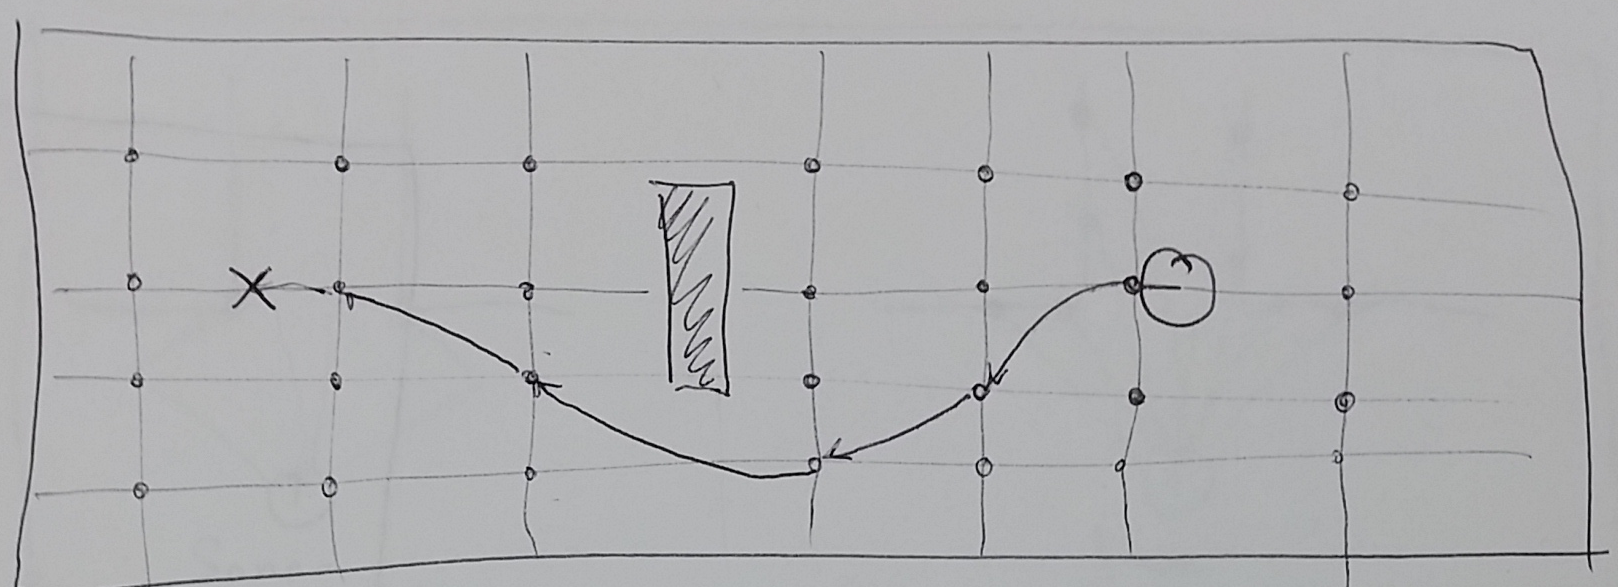
\includegraphics[width=\textwidth]{lattice_rough1.png}
	\caption
	{A lattice planner is an example of a composite discrete and continuous path planner. The planner
	first plans through a discrete grid and then designs trajectories that bring the robot from each point in the planned discrete grid to the next.}
	\label{fig:lattice1}
\end{figure}

\section{Potential Fields} \label{sec:navpotfields}
Potential fields algorithms are continuous local planners. They work on the concept of modeling the robot as a sort of
charged particle (like an electron) and obstacles in the environment are modeled as having the same polarity of charge as the robot thereby producing a repulsive field pushing the robot away
from them. The goal location in is modeled as having an opposite charge to the robot and thus produces an attractive force, pulling the robot towards it. As the robot moves through
the environment, it detects objects and generates motion commands based on its range and direction. 
\begin{figure}
	\centering
	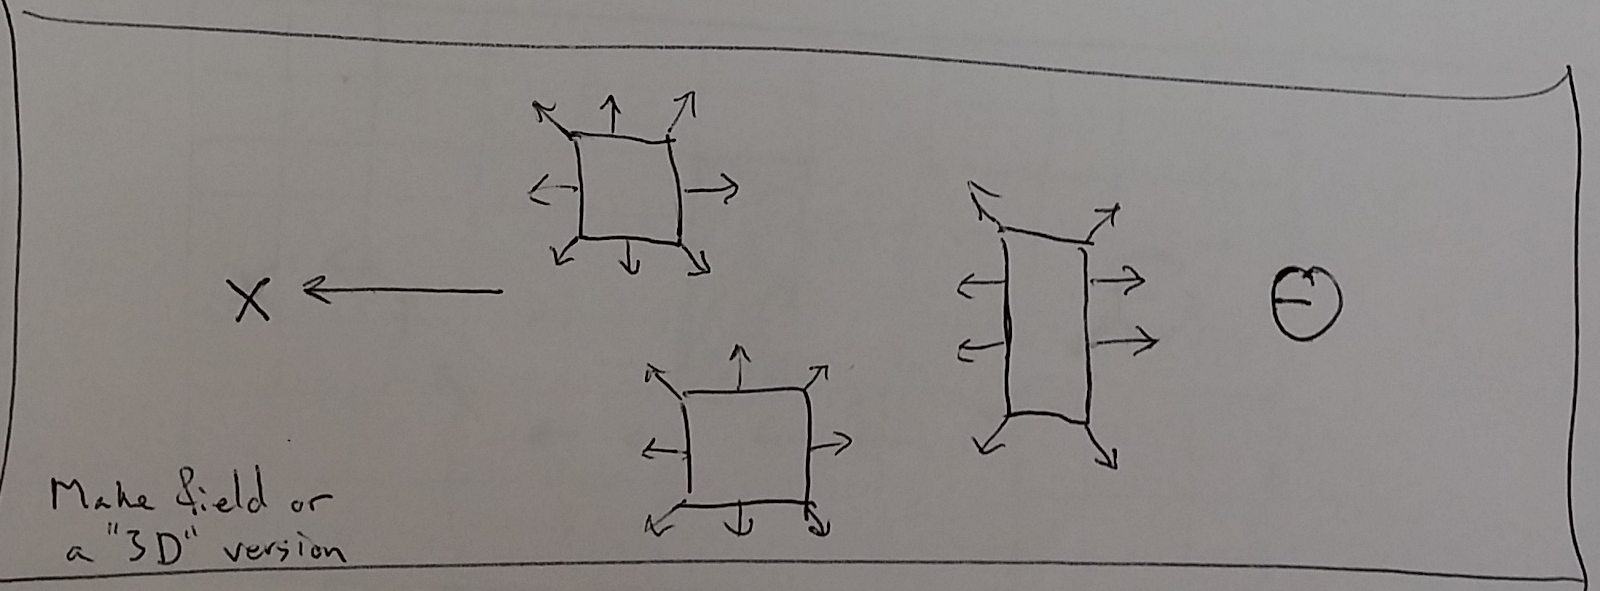
\includegraphics[width=\textwidth]{potentials_rough1.png}
	\caption
	{Visualization of potential fields idea. Objects in the environment emit a field that repels the robot
	 and the goal emits an attractive field. This can be visualized as a 2D or 3D vector field.}
	\label{fig:potentials1}
\end{figure}

Given a vector $x_r$ which describes the position of the robot in the task space and the positions of obstacles
$m_i$ in the set of all obstacles $M$, a force vector $f_i$ can be generated for each obstacle that describes the 
magnitude and direction of the repulsive force applied to the robot by the obstacle. The force direction
is in the opposite direction of the relative bearing of the obstacle to the robot with magnitude being inversely
proportional to the distance of the obstacle from the robot. Equation \ref{eq:potentials_eq1} shows an example
of force vector generation.

\begin{align}
	\norm{f_i}  &= \frac{-c_i}{\norm{m_i - x_r}^\alpha}\\
	\angle{f_i} &= \angle(m_i - x_r)
\label{eq:potentials_eq1}
\end{align}

$m_i - x_r$ is the location of the obstacle relative to the robot and $c_i$ is a positive scalar used to tune force
magnitude. In some implementations, $c_i$ can be a function of the relative bearing, for example, decreasing the repulsion
effect if the obstacle is not in the direction of the goal. The parameter $\alpha$ in general can be any positive scalar
but is often picked to be 2.

For the goal seeking behavior, the equations are similar, with the direction of the force being in the direction of the 
goal, rather than away from it.

\begin{align}
	\norm{f_g}  &= \frac{c_g}{\norm{x_g - x_r}^\gamma}\\
	\angle{f_g} &= \angle(x_g - x_r)
\label{eq:potentials_eq2}
\end{align}

$x_g - x_r$ in equation \ref{eq:potentials_eq2} is the relative location of the goal with respect to the robot and $c_g$ is some positive
tuning scalar. $\gamma$ is some positive scalar, typically 2.

The sum of these forces is used to produce a force vector $f_r$ used to command the robot away from obstacles and towards the goal
location. 

\begin{equation}
	f_r = f_g + \sum_{i = 1}^{\norm{M}} f_i
\label{eq:potentials_eq3}
\end{equation}

where $\norm{M}$ is the number of obstacles (modeled as a discrete set).

\section{GODZILA} \label{sec:navgodzila}

GODZILA (Game-theoretic Optimal Deformable Zone with Inertia and Local Approach) \cite{Krishnamurthy07} is a local 
continuous navigation algorithm based on the potential fields idea. In contrast to some potential fields formulations
which work on the range and bearing of objects in the environment, GODZILA uses the sensor information about occlusion
locations directly in order to formulate navigation commands. It is a memoryless algorithm and does not attempt to
build a map of the environment making it very lightweight in terms of both computation and memory. It can be implemented
on a variety of vehicles and is suited for the cases where a low computational power microcontroller is utilized.
It has three components which are an optimization cost, a straight line planner, and a stochastic local minima escape strategy.

Figure \ref{fig:godzila_setup1} illustrates the key variables in the formulation.
\begin{figure}
	\centering
	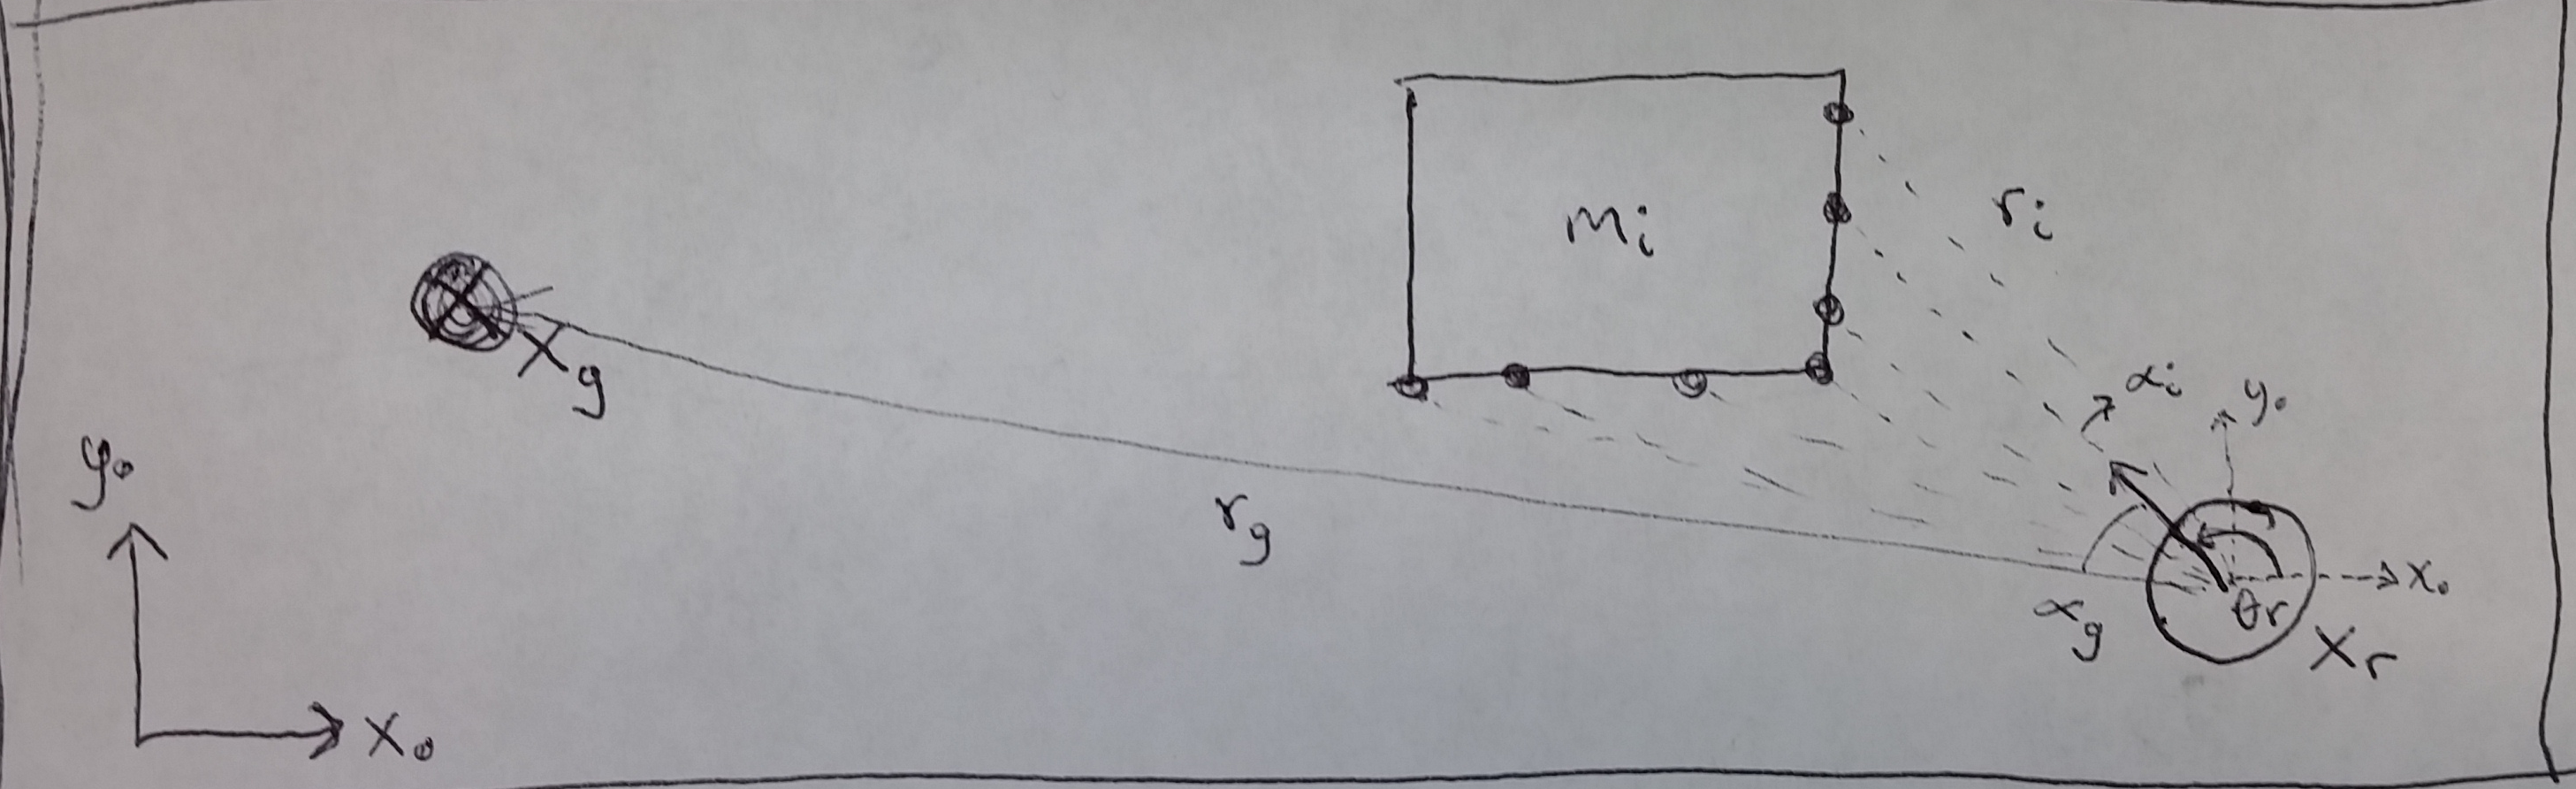
\includegraphics[width=\textwidth]{godzila_rough1.png}
	\caption
	{Illustration of various variables utilized in GODZILA. Range and bearing of the goal relative to the robot are required
	 as well as being able to take range measurements to occlusions and knowing the relative bearings of these measurements.}
	\label{fig:godzila_setup1}
\end{figure}

Taking a 2D example of the application of the GODZILA algorithm, we have the following terms:

\begin{description}
	\item[$x_0$] is the x-axis of the inertial frame.
	\item[$y_0$] is the y-axis of the inertial frame.
	\item[$x_r$] is the (x,y) location of the robot in the inertial frame.
	\item[$\alpha_r^\prime$] is the new heading the robot should be commanded to in the robot frame.
	\item[$x_g$] is the (x,y) location of the goal in the inertial frame.
	\item[$r_g$] is the range to the goal relative to the position of the robot.
	\item[$\alpha_g$] is the bearing to the goal location relative to the orientation of the robot.
	\item[$z_i$] is the $i^{th}$ sensor measurement made by the robot which includes range and bearing to an occlusion.
	\item[$r_i$] is the $i^{th}$ range measurement to an occlusion relative to the position of the robot.
	\item[$\alpha_i$] is the bearing angle to the $i^{th}$ sensor measurement.
\end{description}

In this formulation, it is assumed that there is some mechanism to allow the robot to get an estimate of the relative
range and bearing to the goal location $r_g$ and $\alpha_g$ and that the robot has some sensors that can provide range
and bearing to occlusions in the environment.

\subsection{Optimization Formulation} \label{subsec:navoptimization}
The formulation of the GODZILA algorithm is in terms of an optimization cost. The goal of the algorithm is to bring the robot
towards the goal while preventing it from colliding with obstacles. With this intuition the cost function has three components:

\begin{enumerate}
	\item $J_1(\alpha_r^\prime)$ which rewards goal seeking by penalizing directions other than those towards the goal.
	\item $J_2(\alpha_r^\prime)$ which penalizes directions towards occlusions.
	\item $J_3(\alpha_r^\prime)$ which dampens oscillations by penalizing changes in heading.
\end{enumerate}

The sum of these terms produces the cost function to be minimized:

\begin{equation}
	\min_{\alpha_r^\prime} \sum_{i = 1}^3 J_{i}(\alpha_r^\prime)
\end{equation}

where $\alpha_r^\prime$ is the heading direction the robot should travel in order to minimize the cost function. 
$J_1(\alpha_r^\prime)$ takes on the form of:
\begin{equation}
	J_1(\alpha_r^\prime) = g_{11}(r_g) f_{11}( \norm{\alpha_r^\prime - \alpha_g} ).
\end{equation}

$g_{11}$ is a class-${\cal L}$ function meaning that it is continuous and monotonically non-increasing which maps $[0, \infty) \mapsto [0,\infty)$
and $f_{11}$ is a class-${\cal K}$
function meaning it is monotonically non-decreasing which maps $[0, \infty) \mapsto [0,\infty)$. 
The intuition here is that $f_{11}$ produces a higher cost in proportion to how much the direction command $\alpha_r^\prime$ differs from the goal direction.
$g_{11}$ conversely reduces the cost if the range to the goal is large. The idea being that the farther from the goal the robot is, then being oriented
towards the goal becomes less of a priority. 

$J_2(\alpha_r^\prime)$ takes on the form:
\begin{align}
	J_2(\alpha_r^\prime) &= J_{2_{{\cal I}_1}}(\alpha_r^\prime) - J_{2_{{\cal I}_2}}(\alpha_r^\prime) \label{eq:j2}\\
	J_{2_{{\cal I}_1}}(\alpha_r^\prime) &= \sum_{i \in {\cal I}_1} g_{21}(r_i)\Big [ g_{22}(\norm{\alpha_g - \alpha_i}) + g_{23}(\norm{\alpha_i}) \Big ] g_{24}( \norm{\alpha_r^\prime - \alpha_i}) 
	\label{eq:j2_i1}\\
	J_{2_{{\cal I}_2}}(\alpha_r^\prime) &= \sum_{i \in {\cal I}_2} f_{21}(r_i) g_{25}(\norm{\alpha_g - \alpha_i}) g_{26}( \norm{\alpha_r^\prime - \alpha_i}) \label{eq:j2_i2} 
\end{align}

Equation \ref{eq:j2} has two components to it, separated by the membership of the sensor measurements $z_i$ to one of two sets. 
The first is the set of all range measurements $r_i$ whose value falls below some positive scalar $r_c$ are put into a set ${\cal I}_1$. 
The second set is the remaining range measurements, which are necessarily greater than $r_c$, placed into set ${\cal I}_2$. 
This threshold distance $r_c$ is picked such that if the occlusion is farther away than it, the robot does not need to be concerned with avoiding it.
% J1_I1 = Go away from occlusions that are close to me. Avoid more if they are near my direction of travel or if they are in the direction of the goal.
Equation \ref{eq:j2_i1} is concerned with the occlusions that need to be avoided, and has four class-$\cal L$ functions $g_{21}, g_{22}, g_{23}, g_{24}$ 
associated with it. The first three $g_{21}, g_{22}, g_{23}$ act as gains that the control variable $\alpha_r^\prime$ in function $g_{24}$ must attenuate.
$g_{21}$ says that if the range $r_i$ to the occlusion is small, then the cost of orienting in that direction is high.
$g_{22}$ amplifies this effect if the direction to the occlusion $\alpha_i$ is in the same direction of the goal $\alpha_g$.
$g_{23}$ also amplifies $g_{21}$ if the direction of the occlusion is similar to the heading direction of the robot.
% J1_I2 = Go towards occlusions that are far away and in the direction of the goal.
Equation \ref{eq:j2_i2} deals with the case where the occlusions can be approached. It has one class-${\cal K}$ function $f_{21}$ and two
class-${\cal L}$ functions $g_{25}$ and $g_{26}$. $f_{21}$ and $g_{25}$ act as gains on the controlled function $g_{26}$.
$f_{21}$ promotes moving in the direction of ranges that are large and $g_{25}$ promotes moving in the direction of occlusions
that are in a similar direction to the goal direction. 

The final term $J_3(\alpha_r^\prime)$ is a class-${\cal K}$ function that penalizes changes in direction.

\begin{equation}
	J_3(\alpha_r^\prime) = f_{31}(\norm{\alpha_r^\prime})
	\label{eq:j3}
\end{equation}

This term is present to prevent high frequency oscillations and is analogous to giving the robot a physical inertia.
All of the functions $f_{11}, f_{21}, f_{31}, g_{11}, g_{21}, g_{22}, g_{23}, g_{24}, g_{25}, g_{26}$ in the optimization are tunable by the designer but
it was noted in \cite{Krishnamurthy07} that in the case where the controlled functions $f_{11}, g_{24}, g_{26}, f_{31}$ are 
chosen to be quadratic, the optimization problem can be solved in closed form producing the solution seen in equation \ref{eq:closed_form1}.

\begin{align}
	\alpha_r^\prime &= \frac{\alpha}{\norm{\alpha}} \label{eq:closed_form1} \\
	\alpha &= \alpha_1 + \alpha_2 + \alpha_3 + \alpha_4 \label{eq:closed_form2}
\end{align}

The four terms in equation \ref{eq:closed_form2} correspond to terms arising from the four optimization terms $J_1(\alpha_r^\prime), J_{2_{{\cal I}_1}}(\alpha_r^\prime), J_{2_{{\cal I}_2}}(\alpha_r^\prime), J_3(\alpha_r^\prime)$.
They are expanded in equations \ref{eq:closed_form3}-\ref{eq:closed_form6}.

\begin{align}
	\alpha_1 &= \overline f_{11}g_{11}(r_g)\alpha_g \label{eq:closed_form3} \\
	\alpha_2 &= - \overline g_{24} \sum_{i \in {\cal I}_1} g_{21}(r_i)\Big [ g_{22}(\norm{\alpha_g - \alpha_i}) + g_{23}(\norm{\alpha_i}) \Big ] \alpha_i
					\label{eq:closed_form4} \\
	\alpha_3 &= \overline g_{26} \sum_{i \in {\cal I}_2} f_{21}(r_i) g_{25}(\norm{\alpha_g - \alpha_i})\alpha_i \label{eq:closed_form5} \\
	\alpha_4 &= \overline f_{31} \alpha_r \label{eq:closed_form6}
\end{align}

The solutions to the equations reuse functions $f_{21}, g_{11}, g_{21}, g_{22}, g_{23}, g_{25}$ as they are not functions of $\alpha_r^\prime$ and produce constant versions
of $f_{11}, f_{31}, g_{24}, g_{26}$ as $\overline f_{11}, \overline f_{31}, \overline g_{24}, \overline g_{26}$ in the direction of their respective directions
$\alpha_g, \alpha_i \forall i \in {\cal I}_1, \alpha_i \forall i \in {\cal I}_2, \alpha_r$ where $\alpha_r = [1,0]^T$ representing the current heading of 
the robot in the vehicle frame.

The resultant $\alpha_r^\prime$ is typically commanded as an angular rate $\dot \alpha_r^\prime$ according to the angular velocity bandwidth of the vehicle.

Finally, the linear velocity is still to be commanded. A good choice for this function is of the form:
\begin{equation}
	v_r = f_v(\min(R))g_v(\dot \alpha_r^\prime)
\label{eq:linear_velocity1}
\end{equation}

where $R$ is the set of all range measurements, $f_v$ is a class-${\cal K}$ function and $g_v$ is a class-${\cal L}$ function. 
This reduces the speed of the vehicle when it is in close proximity to occlusions or if it is commanded to a high angular rate.
Slower speeds near obstacles makes it less likely that the vehicle will collide with them. Slower speeds at times when the robot is commanded to
high angular rates helps reduce the distance the robot travels in a previously commanded direction before completing a new 
turn command.

\subsection{Straight Line Planner}

If at some point during the navigation of the vehicle to the goal the straight line path from the robot to goal becomes
unobstructed, it follows that the robot should proceed directly to the goal according to this path. This is sensible, but
can bring the robot in close proximity to obstacles. It is therefore desirable to preserve the obstacle avoidance properties
of the optimization procedure from \ref{subsec:navoptimization}. This procedure is especially useful in situations where the width of the aperture between 
occlusions to the goal approaches the width of the robot where the obstacle avoidance behavior might deter traversal to the goal. 
This can be achieved by prescribing intermediate goal locations
according to:
\begin{equation}
	\hat x_g(t) = (1 - \lambda(t - t_0)) x_r + \lambda (t - t_0) x_g
\label{eq:line_path1}
\end{equation}

where $\lambda(\tau)$ is a monotonically increasing function that maps $[0, T_f] \mapsto [0,1]$ with $T_f$ being some 
amount of time allowed for the vehicle to reach the goal location. The length of time the planner is active is $T_f$.
If the robot has not reached the goal in this time but again has a straight line path to the goal the planner is allowed
to restart.

\subsection{Escape Strategy}

While the inertial term provided by \ref{eq:j3} is intended to reduce high frequency oscillations and backtracking that might
trap the robot in small corners, it is not enough to account for degenerate cases such as those shown in Figure \ref{fig:trap1}.

\begin{figure}
	\centering
	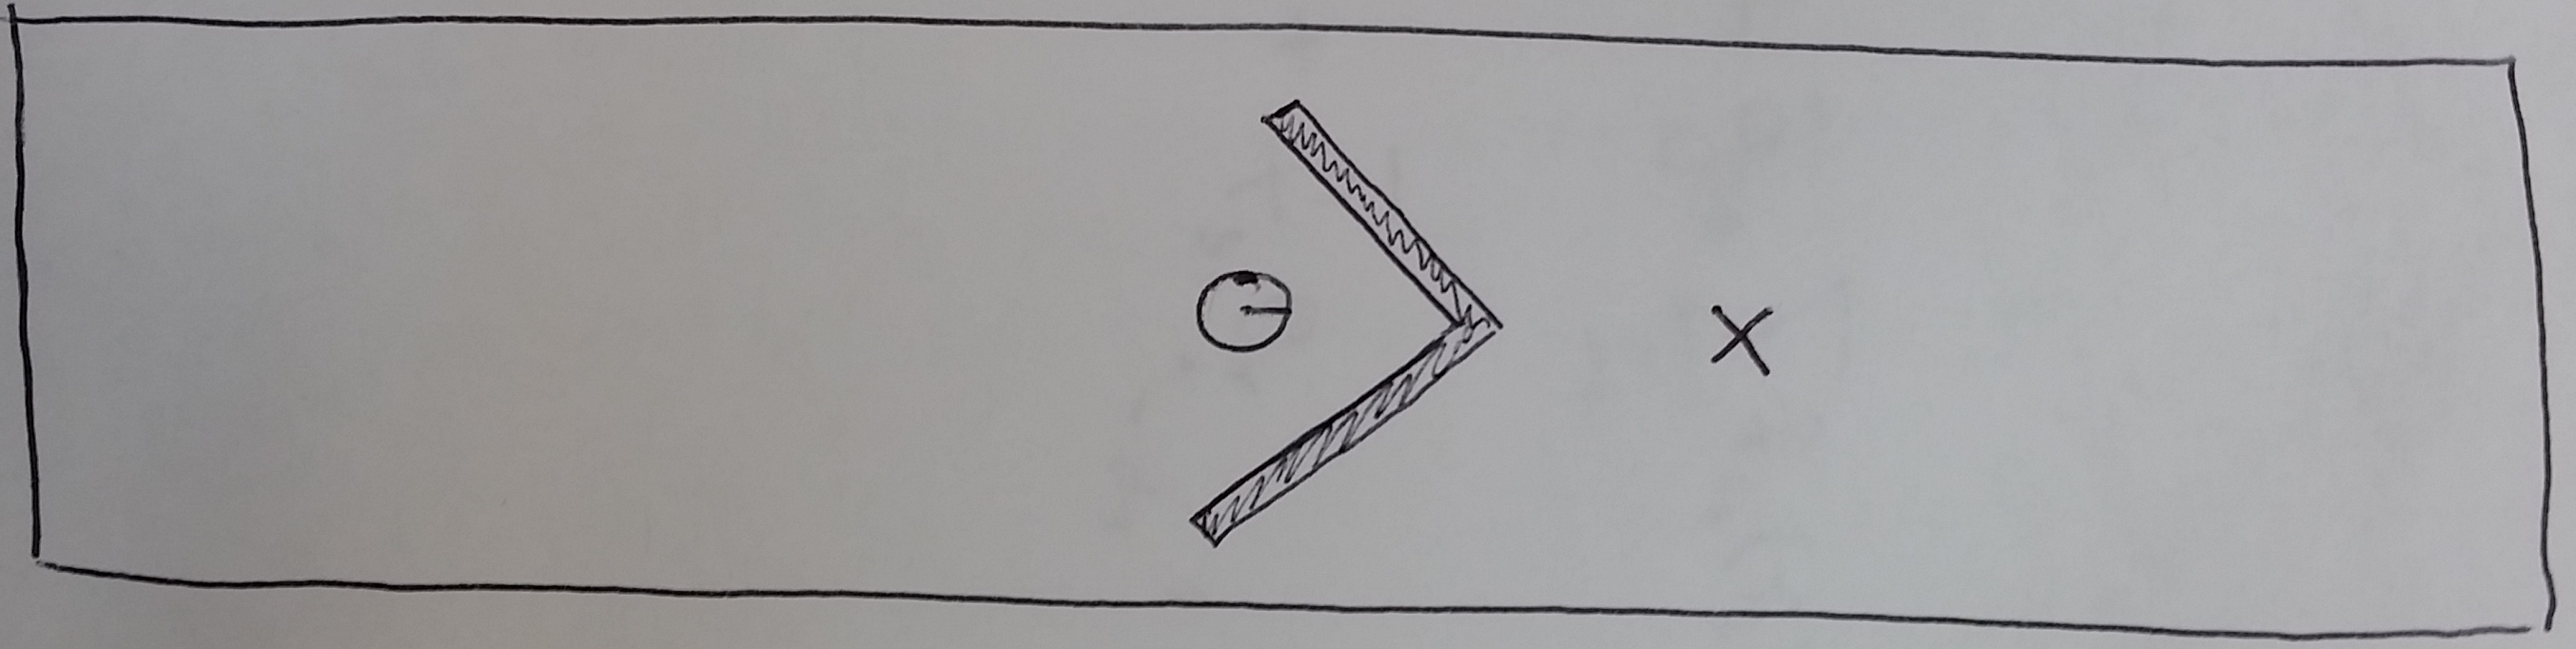
\includegraphics[width=\textwidth]{navtrap1.png}
	\caption
	{A degenerate case where the attractive force of the goal combines with the repulsive force of the wall producing a local optima
	where the robot gets trapped.}
	\label{fig:trap1}
\end{figure}

In such scenarios, an effective strategy to escape such traps is to randomly assign an alternate goal position $x_{rand}$
that will allow the robot to escape the local minima and proceed to the goal. The distance to $x_{rand}$ from the robot
is typically selected to be smaller than the distance to the nearest occlusion $\min(R)$. After some fixed time, the
goal position is set back to $x_g$. If the trap condition is detected multiple times then the next escape procedure is
repeated that many times before being restored to $x_g$. One possible method to detect a trap condition is to integrate
a sliding window of vehicle linear velocities $v_r$ and if those values integrate to a position close to zero then is is likely
that the robot has encountered a trap condition. It is shown in \cite{Krishnamurthy07} that with all of these mechanisms the position of the robot 
$x_r$ will converge to $x_g$ in finite time with probability 1.